\documentclass[12pt]{article}
\usepackage{uwyo_report} % loads in all the specific formatting
\usepackage{amsmath}
\usepackage{amssymb}
\usepackage{float}
\usepackage{multicol}
\setlength{\multicolsep}{6.0pt plus 2.0pt minus 1.5pt}%


% if you want other packages, put them here

% macro for typesetting the word BibTeX
\def\BibTeX{{\rm B\kern-.05em{\sc i\kern-.025em b}\kern-.08em
   T\kern-.1667em\lower.7ex\hbox{E}\kern-.125emX}}


\begin{document}

\title{EE 5450  Project 02: Convolution Neural Network Classification of the Animals Data Set}

\author{David R. Mohler}

%\date{December 7, 1941}

\maketitle

\section{Introduction} 
The rebirth of Neural Networks (NNs) and Machine Learning (ML) has offered revolutionary approaches to intelligent tasks previously unattainable in the field of image processing and computer vision. A major area of research continues to be the automated classification of images. Image classification through classical means of image processing tends to suffer due to problems with the wide variance in images to be classified and how their subject matter may be transformed from image to image. The discovery of Convolution Neural Networks (CNNs) lead to a massive increase in the accuracy of which images could be classified in an automated fashion. 

For this project we will demonstrate the development of several convolution neural networks that vary across a wide number of parameters for the purpose of classifying color images of three different types of animals. The CNN is tasked with classifying images of cats, dogs, and pandas, typical examples of images in the data set can be seen below. Through the variation of network parameters such as the number of layers and the amount of neurons within them, activation functions, learning rates, optimization routines, data augmentation, and other hyper parameters, we display the ability to increase the classification performance of the network. 
\begin{figure}[h]
	\centering % must do this or your figure won't be centered
	\captionsetup{justification=centering}
	\begin{minipage}{0.33\textwidth}
		\centering % must do this or your figure won't be centered
		\includegraphics[width=1\textwidth]{cats_00033.jpg}
	\end{minipage}\hfill
	\begin{minipage}{0.33\textwidth}
		\centering % must do this or your figure won't be centered
		\includegraphics[width=1\textwidth]{dogs_00013.jpg}
	\end{minipage}\hfill
	\begin{minipage}{0.33\textwidth}
		\centering % must do this or your figure won't be centered
		\includegraphics[width=1\textwidth]{panda_00082.jpg}
	\end{minipage}\hfill
\end{figure}

\section{Methods and Results}
After establishing an initial understanding of the basic \pc{ShallowNet} animal classification network that was provided, we begin with a relatively simple and small expansion to include fundamental elements of CNNs, once a working network is established we are able to tune its parameters and observe the effects of varying the optimization techniques. Once a candidate optimizer has been selected we proceed to modify and tune the associated hyperparameters such as the learning rate (when applicable), batch size, number of training epochs, etc. Beyond this we also test the effects of data augmentation. 

\subsection{ShallowNet}
For baseline comparisons we will use the code provided by Dr. Rosebrock \cite{rosebrock} which is a simplistic implementation of a Convolution Neural Network designed with the goal of classification of images in to any of the three given animal categories. The basic structure of Rosebrock's network consists of:
\begin{center}
	\pc{INPUT => CONV => RELU => FC => SOFTMAX} \\
\end{center}
Even with the most basic of implementations, the network is able to provide a respectable first attempt at the classification of the images. As seen in Table \ref{SNR}, the network achieves an average accuracy $66\%$. Given that with three classes the network has a $33\%$ probability of randomly selecting the correct class, this is a decent first attempt. Using this as a lower bound we proceed to implement a number of other techniques that are common in CNN architectures in order to improve the network performance overall. 
\begin{figure}[h]
	\centering % must do this or your figure won't be centered
	\captionsetup{justification=centering}
	\begin{minipage}{0.5\textwidth}
		\centering % must do this or your figure won't be centered
		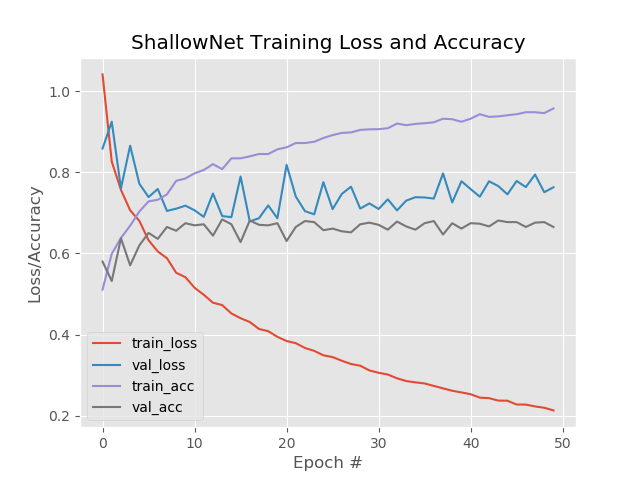
\includegraphics[width=1\textwidth]{BaselineResults_ShallowNet_opt-SGD.png}
		\caption{ShallowNet Accuracy} \label{SN}
	\end{minipage}\hfill
	\begin{minipage}{0.5\textwidth}
		\begin{center}
			\begin{tabular}[2pt]{| c| c| c| c|c|}
				\hline
				& Precision & Recall & F1 & Support \\[0.5ex] 
				\hline 	
				Cat   &    0.64	&0.57&	0.6&	262\\ \hline 
				Dog    &   0.57&	0.58&	0.58&	249\\ \hline 
				Panda   &   0.79&	0.86&	0.82&	239	\\ \hline 
				Avg/Tot  &     0.66 &	0.67 &	0.66 &	750\\ \hline 
				
			\end{tabular}
			\captionof{table}{ShallowNet Results}\label{SNR}
		\end{center}	
	\end{minipage}
\end{figure}
\newpage
\subsection{MohlerNet2}

The initial modification to the original network lies in the expansion of the architecture to incorporate key elements of CNNs, such as pooling layers and data regularization through neuron dropout prior to the fully connected layer. The general architecture of \textbf{``\pc{MohlerNet2}''} is as follows: 
\begin{center}
	\pc{INPUT => CONV => CONV => MAXPOOL => DROPOUT(0.5) => FC => SOFTMAX} \\
\end{center}
More specifically, the CNN employs the use of $3\times3$ kernels in the convolution layers, where the first layer generates 32 feature maps and the second expands to 64 feature maps prior to applying a $2\times2$ max-pooling to the output. From the pooled output a neuron dropout probability of $50\%$ is applied in order to attempt to reduce neuron dependencies and memorization of data. Using the classical stochastic gradient descent (SGD) approach to the optimization of the network we were able to see an immediate and reproducible increase in the ability of the network to accurately classify the three categories of animal images.  From Table \ref{MNR}, it can be seen that the inclusion of the additional convolutional layer, pooling, and dropout was able to provide a $6\%$ increase in the accuracy of the network. For this experiment we used the keras recommended learning rate ($LR = 0.01$). As a more objective measure of the algorithm we can view the F-1 score for each tested network. The F-1 score captures information regarding the false positives and false negatives in the classification process, this gives a more objective view from algorithm to algorithm . From this we can also see a similar increase in F-1 score between the original ShallowNet implementation and the first implementation of MohlerNet (MohlerNet2). 

\begin{figure}[h]
	\centering % must do this or your figure won't be centered
	\captionsetup{justification=centering}
	\begin{minipage}{0.5\textwidth}
		\centering % must do this or your figure won't be centered
		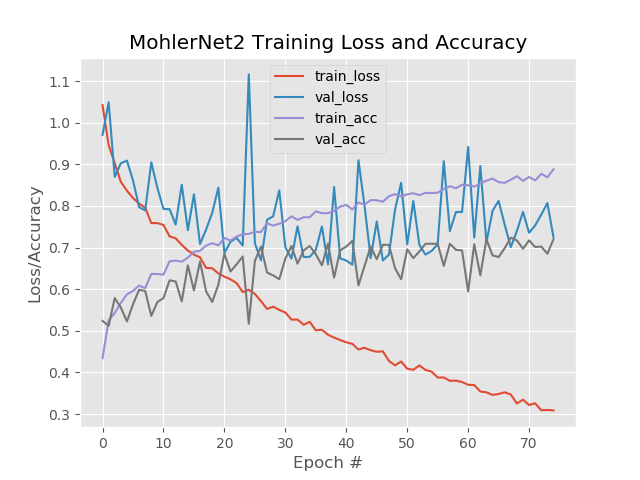
\includegraphics[width=1\textwidth]{MohlerNet2_opt-SGD_KEEP.png}
		\caption{MohlerNet2 Accuracy, Learning Rate:0.01} \label{MN2}
	\end{minipage}\hfill
	\begin{minipage}{0.5\textwidth}
		\begin{center}
			\begin{tabular}[5pt]{| c| c| c| c|c|}
				\hline
					& Precision & Recall & F1 & Support \\[0.5ex] 
				\hline 	
				 Cat   &    0.67  &    0.75   &   0.71   &    262\\ \hline 
				 Dog    &   0.64    &  0.60   &   0.62   &    249\\ \hline 
				 Panda   &    0.88   &  0.82 &     0.85  &     239\\ \hline 
				 Avg/Tot  &     0.72    &  0.72 &     0.72    &   750\\ \hline 

			\end{tabular}
			\captionof{table}{MohlerNet2 Classification Results}\label{MNR}
		\end{center}	
	\end{minipage}
\end{figure}

Once the first trials of the SGD optimized results were obtained we observed the effect of modifying the optimizer for the network. While using the AdaGrad and Adam optimizers, which apply adaptive learning rates, we saw no improvement in any of the scoring metrics. Actually, there was a reduction in accuracy from the original SGD approach, down to an average of approximately $70\%$ classification accuracy. In order to attempt to increase the accuracy of the network we must take in to account that we are dealing with a relatively small data set (by modern standards). With the small number of images being used to train the network there is a high probability that we will experience over-fitting while attempting to increase performance. In order to counter this, we next applied data augmentation to the training set. This allows us to modify the images in moderate ways (rotations, flips, sheering, etc.) such that they are presented to the network in a new way each epoch. Included with this approach was the shift to presentation of the data in batches. a wide variation of batch sizes were tested, anywhere from 16 to 96. Through testing it is heuristically determined that batches of 16 patterns tended to offer better results. The inclusion of data augmentation yielded another (relatively) considerable increase in accuracy and F1-Score. As shown in Table \ref{MN2RAug}, both metrics increased by $4\%$ such that the MohlerNet2 implementation could classify with $76\%$ accuracy. However, from Figure \ref{MN2Aug} it can be seen that from the gap between training accuracy and validation accuracy, the network is experiencing some mild over fitting, which indicates that some modifications may be able to improve the performance further, these remain to be discovered.

\begin{figure}[h]
	\centering % must do this or your figure won't be centered
	\captionsetup{justification=centering}
	\begin{minipage}{0.5\textwidth}
		\centering % must do this or your figure won't be centered
		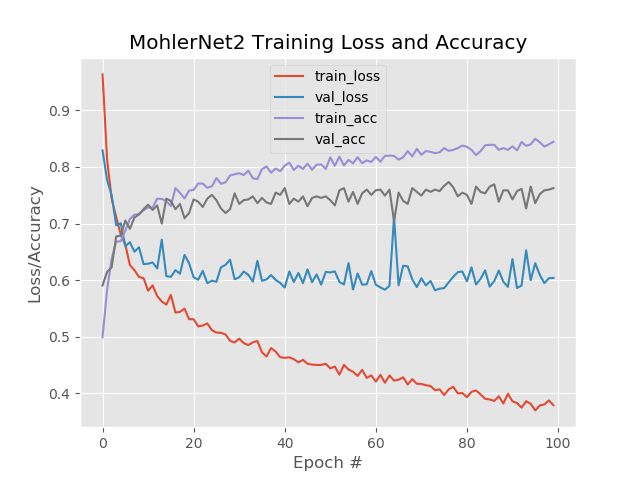
\includegraphics[width=1\textwidth]{MohlerNet2_opt-AdaGradAugment_KEEP.png}
		\caption{MohlerNet2 with Data Augmentation Accuracy, AdaGrad Optimized} \label{MN2Aug}
	\end{minipage}\hfill
	\begin{minipage}{0.5\textwidth}
		\begin{center}
			\begin{tabular}[5pt]{| c| c| c| c|c|}
				\hline
				& Precision & Recall & F1 & Support \\[0.5ex] 
				\hline 	
				Cat   &    0.75&	0.66&	0.71&	262\\ \hline 
				Dog    &   0.69&	0.7&	0.69&	249\\ \hline 
				Panda   &   0.84&	0.93&	0.89&	239\\ \hline 
				Avg/Tot  &    0.76&	0.76&	0.76&	750\\ \hline 
				
			\end{tabular}
			\captionof{table}{MohlerNet2 with Data Augmentation Results}\label{MN2RAug}
		\end{center}	
	\end{minipage}
\end{figure}

\subsection{MohlerNet3}
The next generation implementation of MohlerNet (MohlerNet3) is based upon a simplified version of the layer architecture applied by Alex-Net \cite{NIPS2012_4824}. This iteration has a large increase in layers and number of computations relative to its predecessor. MohlerNet3 employs a total of five convolution layers, the first two layers yield 64 and 128 activation maps respectively, and each layer is paired with its own $2\times2$ max-pooling operation. The following convolution layers use 64, 32 and 32 activation maps respectively with a single $2\times2$ max-pooling at their completion. From here we flatten and regularize the data with a dropout operation with a probability of $50\%$ and apply the standard softmax activation to recieve the output class probabilities. A summary of this network topology is shown below. 
\begin{center}
	\pc{INPUT => [CONV => MAXPOOL]*2 => CONV*3 => MAXPOOL => DROPOUT(0.5) => FC => SOFTMAX} \\
\end{center}
\newpage
In initial experimentation with the learning rate we encountered the effect of a rate which is too large for the network to cope with. As shown in Figure \ref{MN3Fail}, with a learning rate of $\eta = 0.2$ the network diverges. This results in the network accuracy plummeting to $33\%$ which, with three classes is the equivalent of randomly selecting a class. In this case no learning occurs and the propagation of the error through the network in order to correct for the gradient fails. 
\begin{figure}
	\centering % must do this or your figure won't be centered
	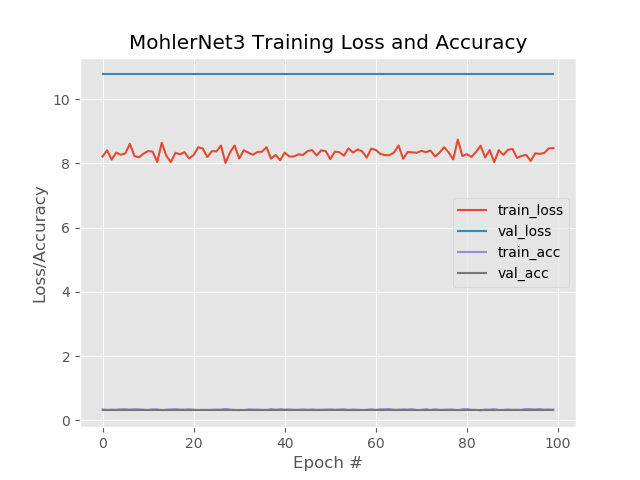
\includegraphics[width=0.5\textwidth]{MohlerNet3_opt-Divergent.png}
	\caption{MohlerNet3 with LR=0.2} \label{MN3Fail}
\end{figure}
As found with the previous iteration, when the network is trained without the application of data augmentation there is a loss of performance. MohlerNet3 obtained an accuracy of $71\%$, and as such its complete results have not been included here. However, when the data is augmented the accuracy of the network is boosted to a value of $77\%$, however, the F1 and recall scores fell slightly, which indicates this network is more subject to false positives and false negatives. 
\begin{figure}[h]
	\centering % must do this or your figure won't be centered
	\captionsetup{justification=centering}
	\begin{minipage}{0.5\textwidth}
		\centering % must do this or your figure won't be centered
		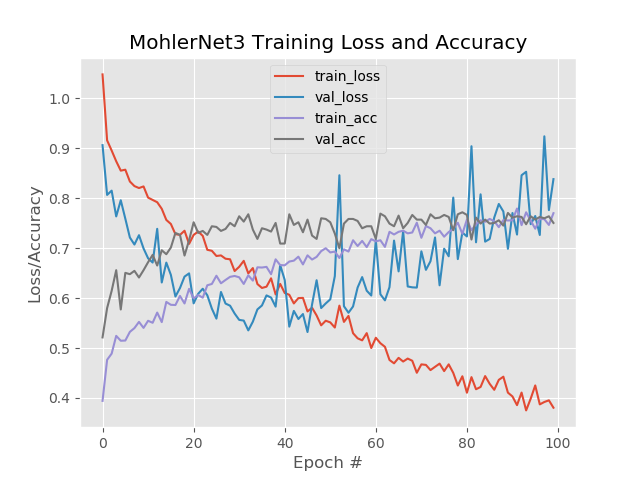
\includegraphics[width=1\textwidth]{MohlerNet3_opt-AdamaxAugmented_KEEP.png}
		\caption{MohlerNet3 with Data Augmentation Accuracy, AdaMax Optimized} \label{MN3Aug}
	\end{minipage}\hfill
	\begin{minipage}{0.5\textwidth}
		\begin{center}
			\begin{tabular}[5pt]{| c| c| c| c|c|}
				\hline
				& Precision & Recall & F1 & Support \\[0.5ex] 
				\hline 	
				Cat   &    0.81&      0.58 &     0.68  &     262\\ \hline 
				Dog    &   0.62 &     0.78 &     0.69 &      249    \\ \hline 
				Panda   &   0.88&      0.91  &    0.89  &     239   \\ \hline 
				Avg/Tot  &    0.77 &     0.75   &   0.75   &    750\\ \hline 
				
			\end{tabular}
			\captionof{table}{MohlerNet3 with Data Augmentation Results}\label{MN3RAug}
		\end{center}	
	\end{minipage}
\end{figure}

\subsection{MohlerNet4}

Applying what has been discovered in the first two editions of MohlerNet, we modify the architecture of the network into a medium sized network (relative to the first two) which balances a low number of layers with the aim of the higher accuracy provided by the larger of the two networks. From this we select the AdaMax optimizer once more and operate under the assumption that the augmentation of the data consistently provides a boost in performance. Using the architecture shown below, we use 32 activation maps in the first two convolution layers with $3\times3$ kernels and $2\times2$ max-pooling, and 64 activation maps in the final convolution layer. However, in this iteration we add an additional fully connected layer prior to the output layer with 64 fully connected neurons.
\begin{center}
	\pc{INPUT => [CONV => MAXPOOL]*3 => FC => DROPOUT => FC => SOFTMAX} \\
\end{center} 
Using the ReLU activation for all layers we achieve results that are comparable to the much larger MohlerNet3 as shown in Table \ref{MN4RAug}.

\begin{figure}[h]
	\centering % must do this or your figure won't be centered
	\captionsetup{justification=centering}
	\begin{minipage}{0.5\textwidth}
		\centering % must do this or your figure won't be centered
		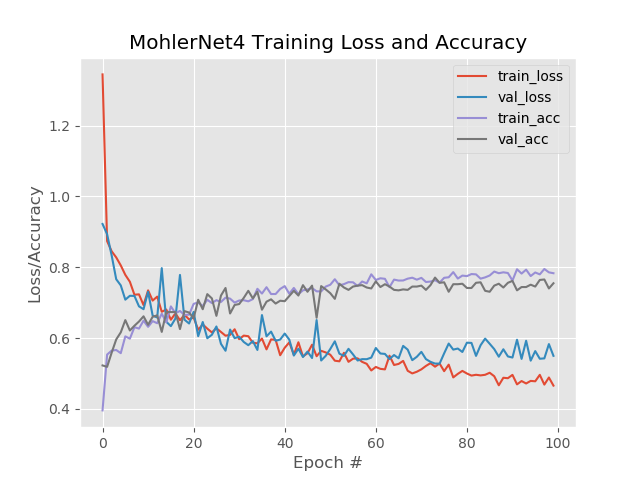
\includegraphics[width=1\textwidth]{MohlerNet4_opt-Adamaxtests.png}
		\caption{MohlerNet4 with Data Augmentation Accuracy, AdaMax Optimized} \label{MN4Aug}
	\end{minipage}\hfill
	\begin{minipage}{0.5\textwidth}
		\begin{center}
			\begin{tabular}[5pt]{| c| c| c| c|c|}
				\hline
				& Precision & Recall & F1 & Support \\[0.5ex] 
				\hline 	
				Cat   &    0.76&	0.61&	0.67&	262\\ \hline 
				Dog    &   0.64&	0.79&	0.71&	249    \\ \hline 
				Panda   &  0.93&	0.92&	0.92&	239  \\ \hline 
				Avg/Tot  &   0.77&	0.77&	0.76&	750\\ \hline 
				
			\end{tabular}
			\captionof{table}{MohlerNet4 with Data Augmentation Results}\label{MN4RAug}
		\end{center}	
	\end{minipage}
\end{figure}

With the promising results delivered by MohlerNet4, we next experimented with the modification of the activation function in the first dense layer. Instead of the use of ReLU as is done in all previous networks and layers, we attempted the use of the hyperbolic tangent activation function. In terms of classification accuracy, this yielded the best network. Edging out the previous best by a single percentage point, we were able to obtain a classification percentage of $78\%$. While this result was able to be replicated to within a single percent, it should be noted that the loss and accuracy characteristics from Figure \ref{MN4Augtanh} are not typical. It can be seen that the validation accuracy out strips the training accuracy by nearly $20\%$, as well as displaying the training loss not approaching the desired value of zero within the trained period. 

\begin{figure}[h]
	\centering % must do this or your figure won't be centered
	\captionsetup{justification=centering}
	\begin{minipage}{0.5\textwidth}
		\centering % must do this or your figure won't be centered
		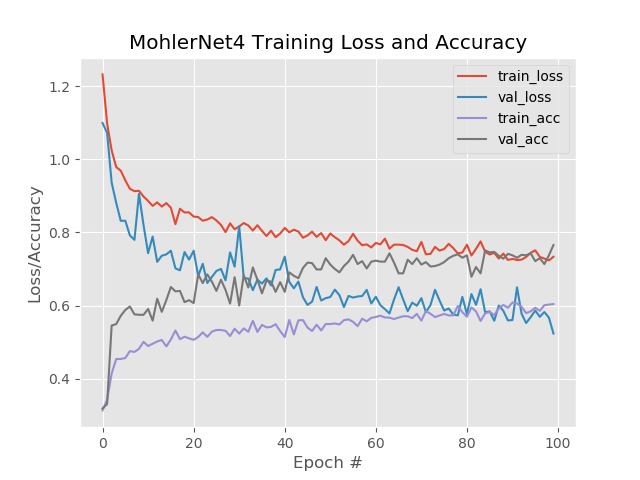
\includegraphics[width=1\textwidth]{MohlerNet4_opt-Adamax.png}
		\caption{MohlerNet4 with Data Augmentation Accuracy, AdaMax Optimized} \label{MN4Augtanh}
	\end{minipage}\hfill
	\begin{minipage}{0.5\textwidth}
		\begin{center}
			\begin{tabular}[5pt]{| c| c| c| c|c|}
				\hline
				& Precision & Recall & F1 & Support \\[0.5ex] 
				\hline 	
				Cat   &    0.83&	0.51&	0.63&	262\\ \hline 
				Dog    &   0.64&	0.83&	0.72&	249   \\ \hline 
				Panda   &   0.85&	0.95&	0.9&	239   \\ \hline 
				Avg/Tot  &   0.78&	0.76&	0.75&	750\\ \hline 
				
			\end{tabular}
			\captionof{table}{MohlerNet4 with Data Augmentation (tanh variant) Results}\label{MN4RAugtanh}
		\end{center}	
	\end{minipage}
\end{figure}
\newpage
\subsection{Network Comparisons}
When comparing the final performances of all three network implementations several factors should be considered, here we will include the raw accuracy, F1 scores, and computational burdens. 
At first pass we can see that each iteration of MohlerNet was able to increase in accuracy, even though it was only for a total of 2\%. In terms of F1 scores the networks were all within a single point from each other, however the difference between the accuracy and F1 score is greatest for MohlerNet4. Lastly, we can look to the number of learn-able weight parameters in the network. As would be expected, the network with the greatest number of layers and applied convolution filters (MohlerNet3) carries the greatest computational burden. This makes it apparent that the expansion of a network to be larger in terms of layers and neurons does not necessarily equate to an increase in task performance. As in all practical engineering tasks there are trade offs to be made in selecting the best network. In terms of raw accuracy it is apparent that MohlerNet4 is the clear winner, however it is 138\% larger than MohlerNet2 in terms of necessary parameters, this directly translates to an increase in computational and memory burden. For a potential implementation it would be necessary to justify a decision for the increased burden for the single percentage of accuracy that is gained from selecting version four over version two. Conversely, it could be said that of the tested networks MohlerNet3 is the worst implementation. While it does provide the mean accuracy it is tied for the lowest F1 score metric and requires nearly double the parameters to accomplish its classification process. These figures are summarized in Table \ref{compare} below.




\begin{center}
	\begin{tabular}[5pt]{| c| c| c| c|}
		\hline
		Network	& Accuracy (\%) &F1 Score& \# of Weights\\[0.5ex] 
		\hline 	
		MohlerNet2& 76 & 0.76 & 68,547  \\ \hline 
		MohlerNet3& 77& 0.75 & 178,691  \\ \hline 
		MohlerNet4& 78&0.75& 94,435  \\ \hline 
	\end{tabular}
	\captionof{table}{Network Metrics}\label{compare}
\end{center}	


\section{Conclusions}
In this project we have demonstrated the ability to construct a number of functional convolution neural networks with the ability to classify images of cats, dogs, and pandas. While the classification is far from perfect, in its best instance MohlerNet4 was able to classify at an accuracy of $78\%$ which is a 12\% increase upon the original ShallowNet CNN that was provided. Due to the small data set provided for training and testing we have shown that data augmentation is an essential method used to boost the accuracy of the network (by as much as 5\% in the tested cases). While each optimizer applied was able to create a convergent network, the AdaMax optimzer proved to offer the greatest performance for each of the three networks, and the Adam optimizer consistently provided a reduction in performance compared to the other optimization schemes. Through multiple iteration and critical parameter tuning, we have demonstrated that a convolution neural network can be successfully taught to recognize and categorize images of animals and from this we have displayed essential pieces of analysis and the necessary design steps to create a functional network.  
\newpage
\appendix % this command sets sectioning command to the appendix format
% uncomment the next line to start on a fresh page



\section{Code Listings}\label{code}

% input the file containing the code
\lstinputlisting[caption={Top Level CNN Implementation},label={MNETop}]{Mohler_CNN.py}
\lstinputlisting[caption={MohlerNet Implementations},label={MNET}]{MohlerNet.py}
%\lstinputlisting[caption={QR Decomp Based Algorithm Implementation},label={alg}]{MonoPoseQR.m} 
%\lstinputlisting[caption={Rearranged QR Decomposition (Credit: Dr. John McInroy)},label={qrCom}]{qrCommute.m}


%% The commands below automatically generate the References section
%% using the ``sample_bib'' file I've given you.

\newpage  % start a new page
\bibliographystyle{ieeetr}
\bibliography{Proj2}

\end{document} % always the last line of your document file
